\documentclass[landscape,a0paper,fontscale=0.34]{baposter}
\usepackage{amssymb}
\usepackage{amsmath}
\usepackage{amsthm}
%\usepackage{amsaddr} % to allow inclusion of institution address
%\usepackage{charter}
\usepackage{enumitem}
\usepackage{graphicx}
\usepackage{wrapfig}
\usepackage{caption}
\usepackage{floatrow}  % to place graph and caption side by side
\usepackage{multicol}
\usepackage{listings}
\usepackage{lipsum}
\usepackage{xcolor}

%\usepackage{subcaption} % for better subcaptions
%\usepackage{verbatim}   % for comment environment
%\usepackage{booktabs}   % for publication-quality tables
%\usepackage{algorithm}  % for the algorithm environment
%\usepackage[flushleft, online]{threeparttable} % for table footnotes
%\usepackage{grffile}

%\usepackage[usenames,dvipsnames]{color} % for highlighting / strikethroughs
%\usepackage{multicol}
\definecolor{boxcolour}{RGB}{139,184,232}
%\definecolor{boxcolour}{RGB}{191, 250, 238}

%%%%%%%%%%%%%%%%%%%%%%%%%%%%%%%%%%%%%%%%%%%%%%%%%%%%%%%%%%%%%%%%%%%%%%%%%%%%%%%%
% Multicol Settings
%%%%%%%%%%%%%%%%%%%%%%%%%%%%%%%%%%%%%%%%%%%%%%%%%%%%%%%%%%%%%%%%%%%%%%%%%%%%%%%%
\setlength{\columnsep}{0.7em}
\setlength{\columnseprule}{0mm}

%%%%%%%%%%%%%%%%%%%%%%%%%%%%%%%%%%%%%%%%%%%%%%%%%%%%%%%%%%%%%%%%%%%%%%%%%%%%%%%%
% Save space in lists. Use this after the opening of the list
%%%%%%%%%%%%%%%%%%%%%%%%%%%%%%%%%%%%%%%%%%%%%%%%%%%%%%%%%%%%%%%%%%%%%%%%%%%%%%%%
\newcommand{\xcompresslist}{%
 \setlength{\itemsep}{1pt}%
 \setlength{\parskip}{0pt}%
 \setlength{\parsep}{0pt}%
}

\newcommand{\compresslist}{%
 \setlength{\itemsep}{5pt}%
 \setlength{\parskip}{0pt}%
 \setlength{\parsep}{0pt}%
}

\newcommand{\compresslistless}{%
 \setlength{\itemsep}{3.25pt}%
 \setlength{\parskip}{0pt}%
 \setlength{\parsep}{0pt}%
}

%Special for paper
\def\phi{\varphi}
\def\by{\mathbf{y}}
\def\bs{\mathbf{\sigma}}
\def\bX{\mathbf{X}}
\def\bB{\mathbf{B}}
\def\bPhi{\mathbf{\Phi}}
\def\brho{\mathbf{\rho}}
\def\pl{p_\lambda}
\def\pln{p_{\lambda_n}}
\def\G{\mathcal{G}}
\def\rto{\leftarrow}
\def\s{\sigma}
\def\o{\omega}
\def\A{\mathcal{A}}
\renewcommand{\th}{\theta}
%\renewcommand{\thh}{\hat{\theta}}
\newcommand{\bth}{\boldsymbol\theta}
\renewcommand{\b}{\beta}
\newcommand{\hb}{\hat{\beta}}
\newcommand{\hbB}{\widehat{\mathbf{B}}}
\newcommand{\hB}{\widehat{B}}
\newcommand{\hO}{\widehat{\Omega}}
\newcommand{\hP}{\widehat{\Phi}}
\newcommand{\hR}{\widehat{R}}
\newcommand{\hT}{\widehat{\Theta}}
\newcommand{\one}{\mathbf{1}}
\def\bn{\boldsymbol\nu}
\def\bu{\mathbf{u}}
\newcommand{\tB}[1]{\widetilde{B}(#1)}
\newcommand{\tOm}[1]{\widetilde{\Omega}(#1)}

%%%%%%%%%%%%%%
\def\estperm{\widehat{\pi}}
\def\dagadjest{\widehat{B}}
\def\goodperm{\pi_{0}}
\def\penderiv{\rho_\lambda'(0+)}


\newcommand{\cemph}[1]{\textcolor{cyan!80!blue}{#1}}
\newcommand{\ccemph}[1]{\textcolor{magenta}{#1}}
\newcommand{\rc}[1]{{\color{red}#1}}
\newcommand{\gc}[1]{{\color{green}#1}}
\begin{document}

\begin{poster}{
 % Show grid to help with alignment
 grid=false,
 columns=3,
 % Column spacing
 colspacing=1em,
 % Color style
 headerColorOne=boxcolour, %gray!20!white!90!black,
 borderColor=boxcolour,
 % Format of textbox
 textborder=rectangle,
 textfont=\sffamily,
 linewidth=0.25mm,
 % Format of text header
 headerborder=closed,
 headershape=rectangle,
 headershade=plain,
 headerfont=\large\rmfamily\bf,
 background=none,
 bgColorOne=gray!90!black,
 boxColorOne=white,
 headerheight=0.12\textheight}

% Title
{\huge GIVE ME YOUR PANDEMIC PLAYLIST:\\[0.2em] A Study of Top 200 Charts Before and After COVID-19}
% Authors
{Victoria Coronado, Chris Lee, Dale Hanks, Matt Turk, Sophia Yang \& Richard Yim
 \\[0.2em]{(Advisor: Vivian Lew \texttt{vlew@stat.ucla.edu})}}
 % University logo
 {
  \begin{tabular}{c}
    
\includegraphics[height=0.09\textheight]{ps_statistics_DoS}%{ucla_cw}
    
\includegraphics[height=0.09\textheight]{Spotify_Logo_RGB_Green}
  \end{tabular}
 }


\headerbox{Introduction}{name=intro,column=0,row=0,span=3}{
Due to the global outbreak of COVID-19, the year 2020 was unique and challenging (to put it briefly). Struggling with fear of infection, possible job loss and/or relocation, and lack of toilet paper, millions underwent substantial emotional turmoil. As humanity searched for ways to cope with the difficulties we faced, many turned to various forms of entertainment, including music, to pass time at home. The purpose of this study is to examine the possibility of a relationship between the effects of the Coronavirus on popular culture, specifically the top 200 songs on Spotify. Naturally, the hottest tracks will always change with time, but it is still possible to analyze the components of each track, and thereby determine what makes it unique. Using data collected from the Spotify top 200 of January 2020 and January 2021, our team examined 765 observations, each with 16 features, which identify the track, tell whether it made the top 200 before or after the beginning of the COVID-19 outbreak, and rate things like energy, proportion of spoken words, and how much the track sounds like it was recorded live, to name a few.
}
%section{Introduction}
% Matt: introduce why this is interesting
    % what are the labels 

\begin{posterbox}[name=features,column=0,row=0,span=1,below = intro]{Features}
%\headerbox{Features}{name=features,column=0,row=0,span=1, below=intro}{
    \compresslistless
% Victoria: correlation heatmap
    % correlated features, why it make sense
    % discuss actual features
\begin{itemize}[noitemsep]
    \item \textbf{label}: response feature revealing if the song reached the top 200 “before” or “after” COVID-19.
    \item The first two features correspond to the name of the track and artist.
	\item The rest are numerical features, most of which are on a scale from 0 to 1.
		\begin{itemize}[noitemsep]
		    \item \textbf{Acousticness}: rates whether the song is acoustic on a 0 to 1 scale.
		    \item \textbf{Danceability}: how suitable a track is for dancing based on a combination of musical elements including tempo, rhythm stability, and overall regularity.
			\item \textbf{Energy}: measurement of noise and speed.
			\item \textbf{Speechiness}: rates the proportion of spoken words included in the track. 
			\item \textbf{Valence}: how musically positive a track is on a scale from 0 to 1.  (0=sad/angry 1=cheerful)
		\end{itemize}
	\item Correlations
		\begin{itemize}[noitemsep]
			\item \textbf{Energy} and \textbf{loudness} = 0.72
				\begin{itemize}[noitemsep]
					\item As \textbf{loudness} \gc{increases}, \textbf{energy} (noise and speed) also \gc{increases}.
				\end{itemize}
			\item \textbf{Energy} and \textbf{acousticness} = -0.54
				\begin{itemize}[noitemsep]
					\item As \textbf{acousticness} \gc{increases}, \textbf{energy} \rc{decreases}.
				\end{itemize}
		\end{itemize}
\end{itemize}

\centering
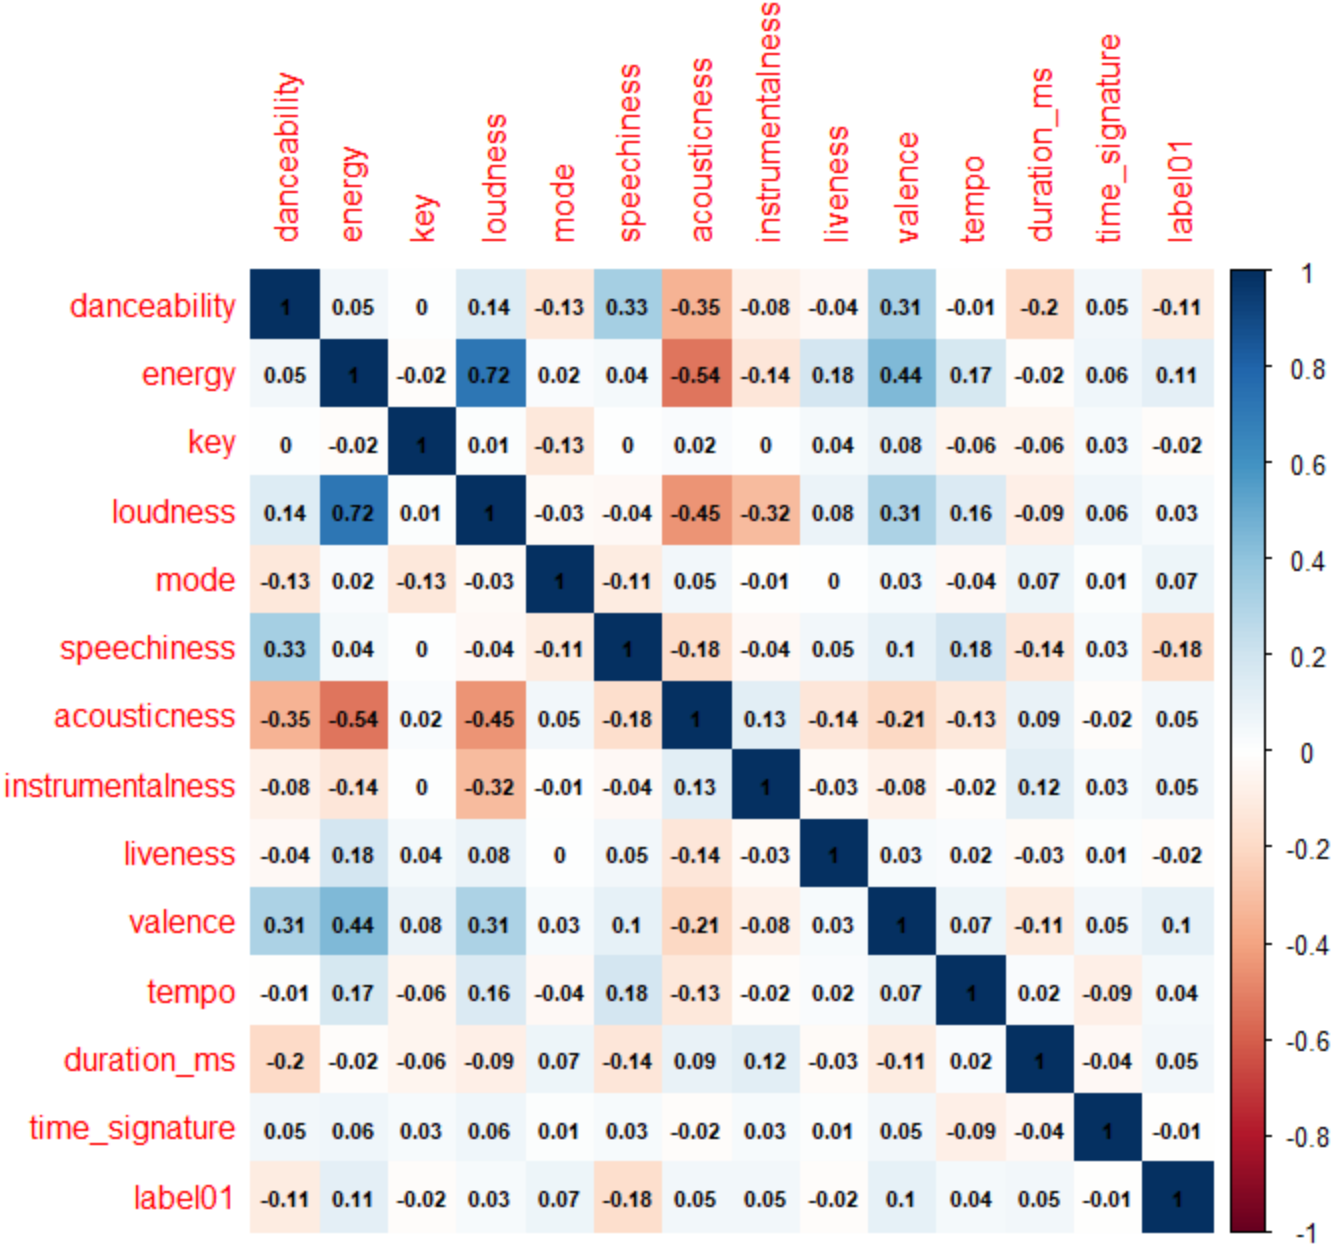
\includegraphics[width=0.9\textwidth]{corrplot2.PNG}
\end{posterbox}



\headerbox{Distribution Difference}{name=dd,column=1,row=0,span=1,below=intro}{
    \compresslistless
% Dale: histograms and discussion why it maters
    % shapes of distributions (skewed, high kurtosis)
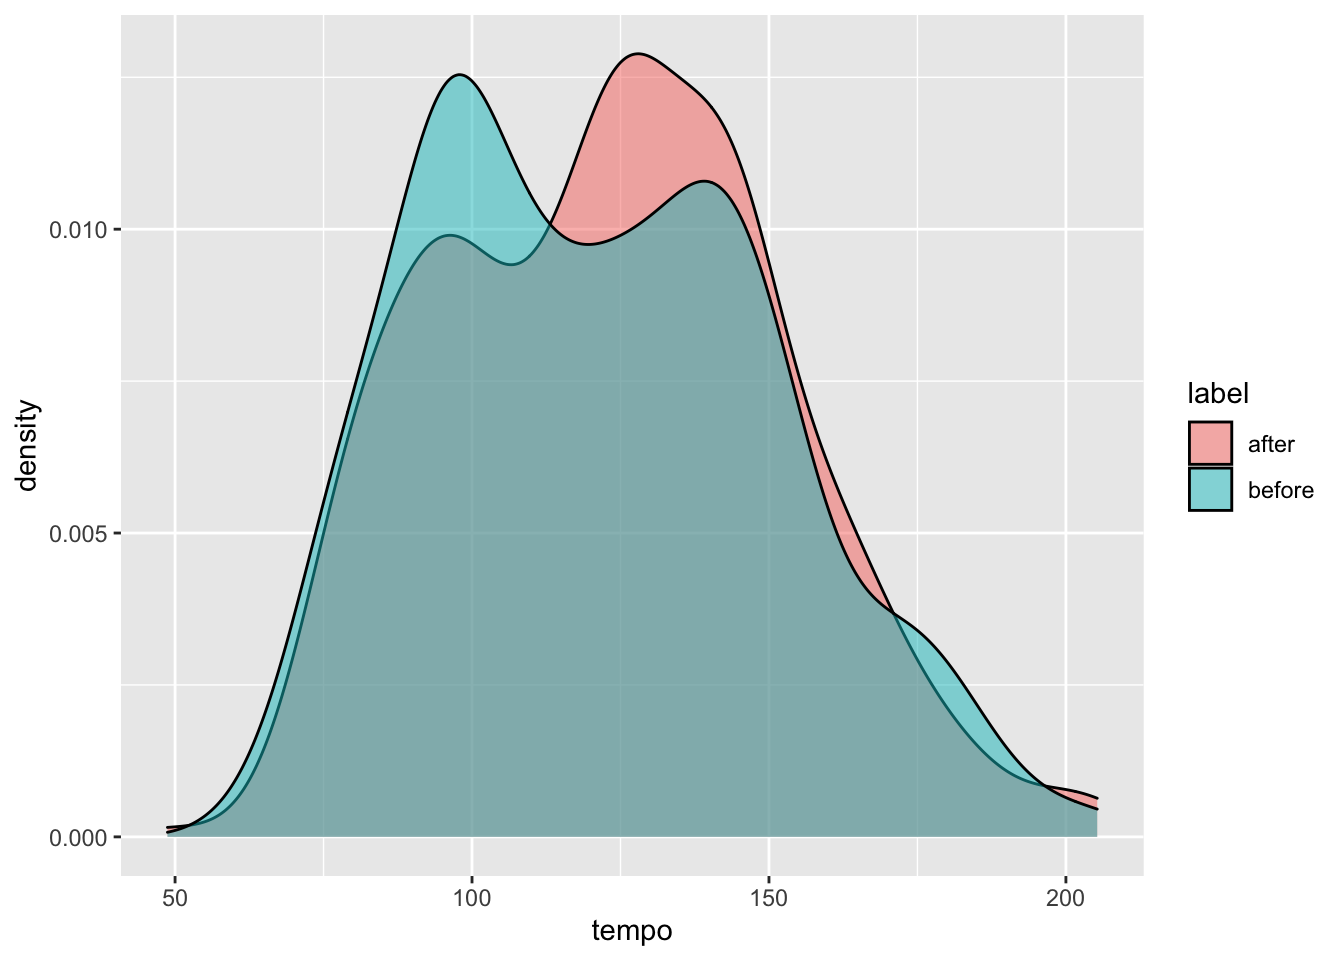
\includegraphics[scale=0.13]{tempo.png}
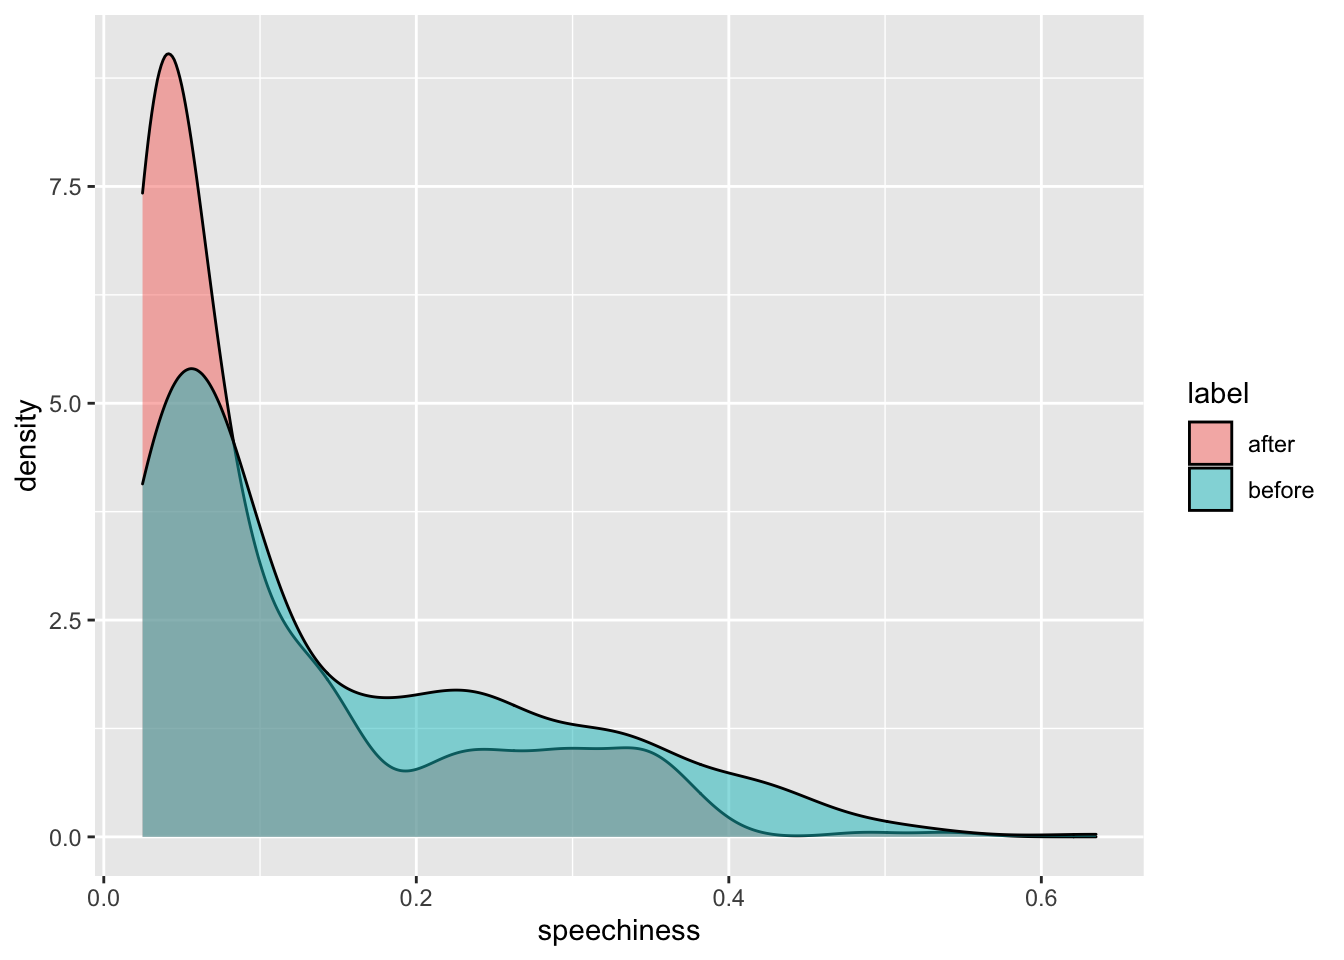
\includegraphics[scale=0.13]{speechiness.png}
Of all our variable histograms, \textbf{tempo} and \textbf{speechiness} show the least amount of overlap. The overall distribution of \textbf{tempo} is rather uniform. However, when splitting the data by \textbf{label}, \textbf{tempo} seems centered around a higher mean for 'after'. The kurtosis for \textbf{tempo before} and \textbf{tempo after} is -0.5922033 and -0.4030732, respectively. This tells us that the center of the distribution is thicker than expected, or that \textbf{tempo} has been consistent to fall within a certain range. The distribution of \textbf{speechiness} is heavily skewed left and shows a much higher density of data in the left region for 'after', even with less observations than 'before'. Two possible reasons could be a shift towards music focused more on the instruments and less on voice, e.g. electronic synthetic music void of vocals and following social distancing guidelines in recording studios.

\vspace{0.3cm}
% Chris: statistical test for sample means wilcoxon rank sum
    % distribution differences that were statistical significant
    % briefly mention how Wilcoxon's, nonparametric test remedy violations of normality *how we circumvent those assumptions*
To find out whether the differences in the top 200 Spotify charts before and after the pandemic are statistically significant, we performed hypothesis testing on song features. We noticed from the histograms that features are not normally distributed except \textbf{duration}. As they do not satisfy the normality under the Gauss-Markov conditions, we used the Wilcoxon rank-sum test as it does not assume any known distributions of our data, it does not deal with parameters, thus it makes an appropriate test for our data. At a 5 percent significant level, we found the differences in \textbf{danceability} (p = 0.00168), \textbf{energy} (0.00335), \textbf{speechiness} (1.082e-08) and \textbf{valence} (0.01068) before and after COVID-19 are statistically significant.
}

\headerbox{Side note: Song Titles}{name = title, column=1,row=0,span=1,below = dd}{
% Sophia: track names, word clouds, frequent title words
    % include word cloud pngs
    % most frequent words
    
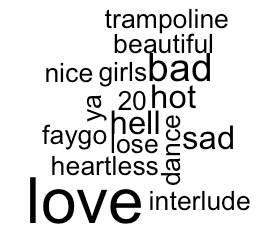
\includegraphics[width=0.4\textwidth]{track_name_before.jpg}
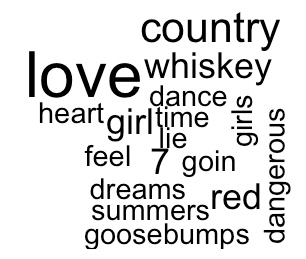
\includegraphics[width=0.4\textwidth]{track_name_after.jpg}

The two wordclouds show that the pandemic has little effect on the most popular song titles, as \textbf{"Love"} remains the top 1 word.
}

\headerbox{Modeling}{name=model,column=2,row=0,span=1,below=intro}{
    \compresslistless
    % Matt: logistic regression
    % three things: energy, speechiness, valence
    % population means for these factors
    
    % Not sure about the format for this part, so I'll just keep it simple for now.
    
    To determine which features were most \underline{instrumental} (pun intended) in predicting whether a track hit the top 200 in 2020 or 2021, we began with a \textif{logistic regression} model. 
    The only three significant predictors are \textbf{energy}, \textbf{speechiness}, and \textbf{valence}. 
    \newline
    A reduced model was trained with the three predictors. 
    Songs in Spotify's top 200 of January 2021 had \underline{higher} \textbf{energy} and \textbf{valence}, while top songs of January 2020 had significantly \underline{higher} \textbf{speechiness}.
    
    \vspace{0.3cm}
    % Richard: gradient boosting 
    Boosting is a general statistical learning approach; we apply boosting using decision trees. Conceptually, boosting iteratively and sequentially grows decision trees by observing the residuals the decisions, in ensemble, during the training process. 
    % tie in with variables found to be significant from logistic regression
     %   \vspace{0.3cm}
    We implement gradient boosting with decision trees using the `gbm` library in `R`. We were interested in achieving a ranking of important variables corresponding to whether or not a song made it to the top 200 charts in the U.S., January 2020 versus January 2021. The gradient boosting process on decision trees naturally does not utilize all variables for each decision tree, so we are able to record a variable importance for how much error we accrue when we leave out a certain variable. We achieved the following ranking of variables after 30 simulations of gradient boosting (we list only the the top five variables):
    \begin{enumerate}
        \item \textbf{Speechiness}, with an average \rc{decrease} (0.152 to 0.109) *
        \vspace{-0.2cm}
        \item \textbf{Energy}, with an average \gc{increase} (0.585 to 0.621) *
        \vspace{-0.2cm}
        \item \textbf{Valence}, with an average \gc{increase} (0.464 to 0.507) *
        \vspace{-0.2cm}
        \item \textbf{Acousticness},  with an average \gc{increase} (0.249 to 0.274)
        \vspace{-0.2cm}
        \item \textbf{Danceability}, with an average \rc{decrease} (0.700 to 0.668) * 
    \end{enumerate}
}

\headerbox{Discussion}{name=dis,column=2,row=0,span=1,below=model}{
    \compresslistless
    % Sophia: wrap everything up, what is interesting in general; limitations of study; extensions
    % *caveat: causal inference being done, this are many possible reasons for this change* 
    % e.g. energy might have increased between 2020 and 2021 
    The two models produce similar results for the feature differences between Top 200 charts in January 2020 vs. 2021. The 2021 ones tend to have fewer words, more energy (noise and speed) and more valence (more musically positive). It makes sense for people to appreciate more energetic and musically positive songs during the COVID-19.\newline
    Still our study has its limitations: we don't have a large dataset with our 765 observations from two months. Also there might be other confounding factors besides the pandemic that are behind this shift in features of top 200 charts.
}

\headerbox{References}{name=ref,column=2,row=0,span=1,below=dis}{
\scriptsize
    Spotify API. \texttt{https://github.com/plamere/spotipy}\newline
   Spotify for Developers, Design Guidelines.
   \texttt{https://developer.spotify.com/documentation/general/\newline design-and-branding/}\newline
   Gareth James et al. \textit{An Introduction to Statistical Learning: with Applications in R}.
   Bo Plantinga. "What do Spotify's audio features tell us about this year's Eurovision Song Contest?" \newline
   \texttt{https://medium.com/@boplantinga/what-do-spotifys-audio-features-tell-us-about-this-year-s-\newline eurovision-song-contest-66ad188e112a}\newline
   Julia Silge, David Robinson. \textit{Text Mining with R: A Tidy Approach}, Ch. 2, Sentiment analysis with tidy data.
   \texttt{https://www.tidytextmining.com/sentiment.html}
}

\end{poster}
\end{document}f